\documentclass{article}

\usepackage{graphicx}
\usepackage{amsmath}
\usepackage{amssymb}
\usepackage[hidelinks]{hyperref}
\usepackage{url}
\usepackage{listings}
\usepackage{caption}
\usepackage{subcaption}
\usepackage{xcolor}

\setlength\parindent{0pt}
\renewcommand{\theenumi}{\alph{enumi}}
\renewcommand{\labelenumi}{\theenumi)}
\lstset{
language=Python,
basicstyle=\ttfamily,
otherkeywords={self},             
keywordstyle=\ttfamily\color{blue!90!black},
keywords=[2]{True,False},
keywords=[3]{ttk},
keywordstyle={[2]\ttfamily\color{yellow!80!orange}},
keywordstyle={[3]\ttfamily\color{red!80!orange}},
emph={MyClass,__init__},          
emphstyle=\ttfamily\color{red!80!black},    
stringstyle=\color{green!80!black},
showstringspaces=false            
}

\title{SAX Acquaintance Report}
\author{Denys \textsc{Sobchyshak}}
\date{\today}

\begin{document}
\maketitle

\section{Introduction}
Symbolic Aggregate approXimation (SAX) is a data reduction technique that not only allows for a drastic decrease in memory use of time series storage, but also enables fast approximate and exact searches in huge amounts of data. This report provides a short description of findings and insights obtained during my acquaintance with SAX \cite{lin2007experiencing} and its further developments in indexable SAX (iSAX) \cite{shieh2008sax} and iSAX 2.0 \cite{camerra2010isax}.

\subsection{Implementation details}
Due to a proof of concept (POC) nature of this work it was decided to use Python as the implementation language, since it facilitates fast solution delivery and incorporates a vast diversity of scientific libraries. The code is also heavily dominated by functional programming style of implementation, since not only such approach is more convenient for handling mathematical concepts, but it also allows more flexibility in terms of further parallelization of the solution.\par
It must be noted, that provided code is far from being optimal due to its POC spirit. Thus, occasional bugs and memory use inefficiencies might be discovered, especially in the graphical interface (GUI) part. However, this should not prevent an informed user from utilizing the solution in its fullest capacity on a modern commodity hardware installation.\par
The following is a list of software installations and libraries, required for the solution to run:
\begin{itemize}
	\item python \textbf{3.4.3}
	\item matplotlib \textbf{1.5.2}
	\item numpy \textbf{1.11.1}
	\item scipy \textbf{0.18.0}
\end{itemize}

\subsection{Definitions}
In the further parts of this work we will refer to SAX as a data reduction technique, however, in some works (e.g. \cite{keogh2001dimensionality}, \cite{lin2007experiencing}, \cite{shieh2008sax} etc.) SAX may be referred to as a dimensionality reduction technique. As implied in \cite{xi2006fast}, I'd like to set a clear boundary between the terms and argue that in a general problem setting SAX is not a dimensionality reduction technique. \par
Specifically, for $n,m,k,l \in \mathbb{N}$ let's define a transformation that receives a $n \times m$ dimensional set with $n$ data points each defined in $\mathbb{R}^m$ and returns a $n \times k$ dataset with $k < m$ and each of $n$ data points defined in $\mathbb{R}^k$ to be a dimensionality reduction technique. Please note, that while according to our definition domains are defined in $\mathbb{R}$, some techniques can use a character space for the domains and we do not wish to exclude those techniques. Given that definition, we will define data or numerosity reduction technique as a transformation that receives $n \times m$ dimensional set with $n$ data points each defined in $\mathbb{R}^m$ and returns a $l \times m$ set, where $l < n$ and the domain of each of $m$ dimensions is arbitrarily defined. \par
Thus, simply put, a data reduction technique provides a different and compressed representation of the original data, yet retains the number of dimensions of the original feature space, while a dimensionality reduction technique tries to find a linear or non-linear combination in the original feature space and reduces that space to only the most important components. However, it can be argued that for a specific problem setting (e.g. nearest neighbor search) SAX can be considered a dimensionality reduction technique.

\section{SAX Representation}
To start with, it was needed to see a SAX representation for a synthetic time series. Thus, it was needed to generate a time series such that it would not require further preprocessing, in other words it would not violate any of SAX assumptions. According to \cite{shieh2008sax} the only assumption SAX makes is that the underlying data has a local Gaussian distribution (i.e. on small intervals), which SAX author claims to be present in over 120 studied data sets from various domains \cite{keogh2006sax_presentation}. Moreover, not only the author claims that the distribution adaptive implementation of SAX that he experimented with would always approximately descend to a Gaussian distribution, but also, even if the underlying data has a different distribution, the SAX approach would still provide valid results only with a degraded performance.\par
Given the aforementioned, a simple random walk with Gaussian distribution for random number generator would provide the needed results and was implemented as
\begin{lstlisting}
import numpy as np
def random_walk(t=1000):
    if t > 0:
        return np.cumsum(np.random.randn(t))
\end{lstlisting}
Furthermore, while SAX algorithm itself is pretty straightforward, the PAA \cite{keogh2001dimensionality} calculation for a non-integer size of the window span turned out to be a bit tricky. It was eventually achieved by scaling the entire domain using the PAA's word length as
\begin{lstlisting}
import numpy as np
def paa(series, w):
    n = len(series)
    series = np.array(series)
    if n == w:
        return series
    if w == 1:
        return [series.mean()]
    if w < 1 or n < w:
        return None
    aggregate = [0]*w
    idx = np.arange(n*w) // w
    for i in range(0, n*w, n):
        aggregate[i//n] = (series[idx[i:i+n]]).sum() / n
    return aggregate
\end{lstlisting}
To showcase the results we will transform two series
$$x1=[ 0.98575863,  0.60495287,  0.83123062, -1.34965375, -1.07228837]$$
$$x2=[-1.24234567, -0.79303633, -0.06255499,  0.49080739,  1.60712961]$$
into their corresponding SAX representations with PAA word length of 4 and SAX cardinality of 5
$$sax1=['100', '100', '010', '001']$$
$$sax2=['001', '010', '100', '100']$$
and measure the distance between them while comparing it to the Euclidean between the original series
$$eucl=4.276009034552973$$
$$mindist=1.965338463812398$$

\section{Alternative Representation}
While reading about dimensionality reduction of time series I've stumbled across a novel technique called forecastability component analysis (ForeCA) \cite{goerg2013forecastable} \cite{goerg2013forecastable_presentation}, which seem to heavily rely on Fourier transforms for spectrum analysis of a series. It's content is rather involving and math intensive, thus was deemed to be out of scope for the purposes of this work. However, as \cite{shieh2008sax} mentioned the use of discrete Fourier transforms (DFT) for data reduction and sequence matching, I decided to investigate the method and implement it accounting for considerations noted in \cite{faloutsos1994fast}.\par
The results were rather interesting and did not follow the recommendations in \cite{faloutsos1994fast} to use only 2-3 frequency components for the aforementioned synthetic time series, but rather required around 100 components for a data set of 2000 points in order to gain reasonable time series reconstruction. However, given that only the frequency components have to be stored, it is still a great reduction from initial time series size. A showcase of DFT reconstruction as compared to the original data can be seen on Figure \ref{fig:1}.
\begin{figure}[h!]
	\begin{center}
		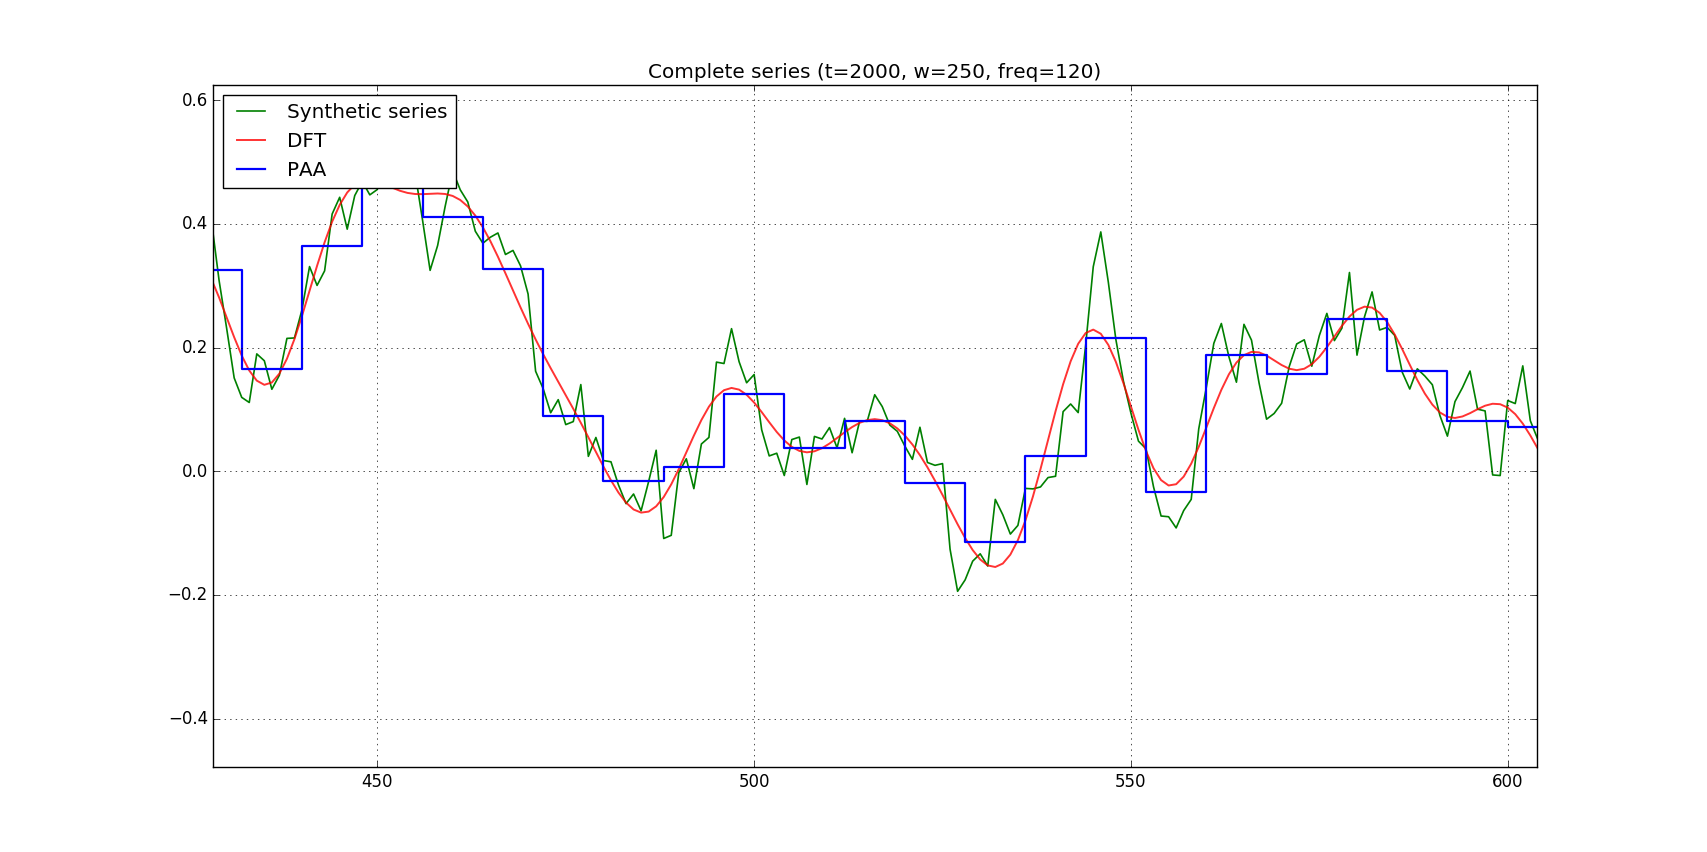
\includegraphics[width=\textwidth]{images/dft-visualization}
		\caption{Comparison of DFT reconstructed and original synthetic time series, where $t$ is the series length, $w$ is the PAA word length and $freq$ is the number of DFT components used}
		\label{fig:1}
	\end{center}
\end{figure}

\section{(Optional) Parallelization}
- argue that this task to a great extent depends on hardware specifications
- give a theoretical explanation of solving this problem
- argue, that for the prototypical purposes of this work it was decided to tangle with py4mpi

\section{Interactive visualization}
For interactive exploration of influence of various parameters on the resulting output as a matplotlib based visualization was implemented. It comprises four visualizations with several parameter control sliders as explained in Figure \ref{fig:2}. In order to interact with the visualization one will need to click on different parts of sliders. Please note, that changing the time series length will result in generation of a new random walk, while change of other parameters only adapts the corresponding transformations.
\begin{figure}[h!]
	\begin{center}
		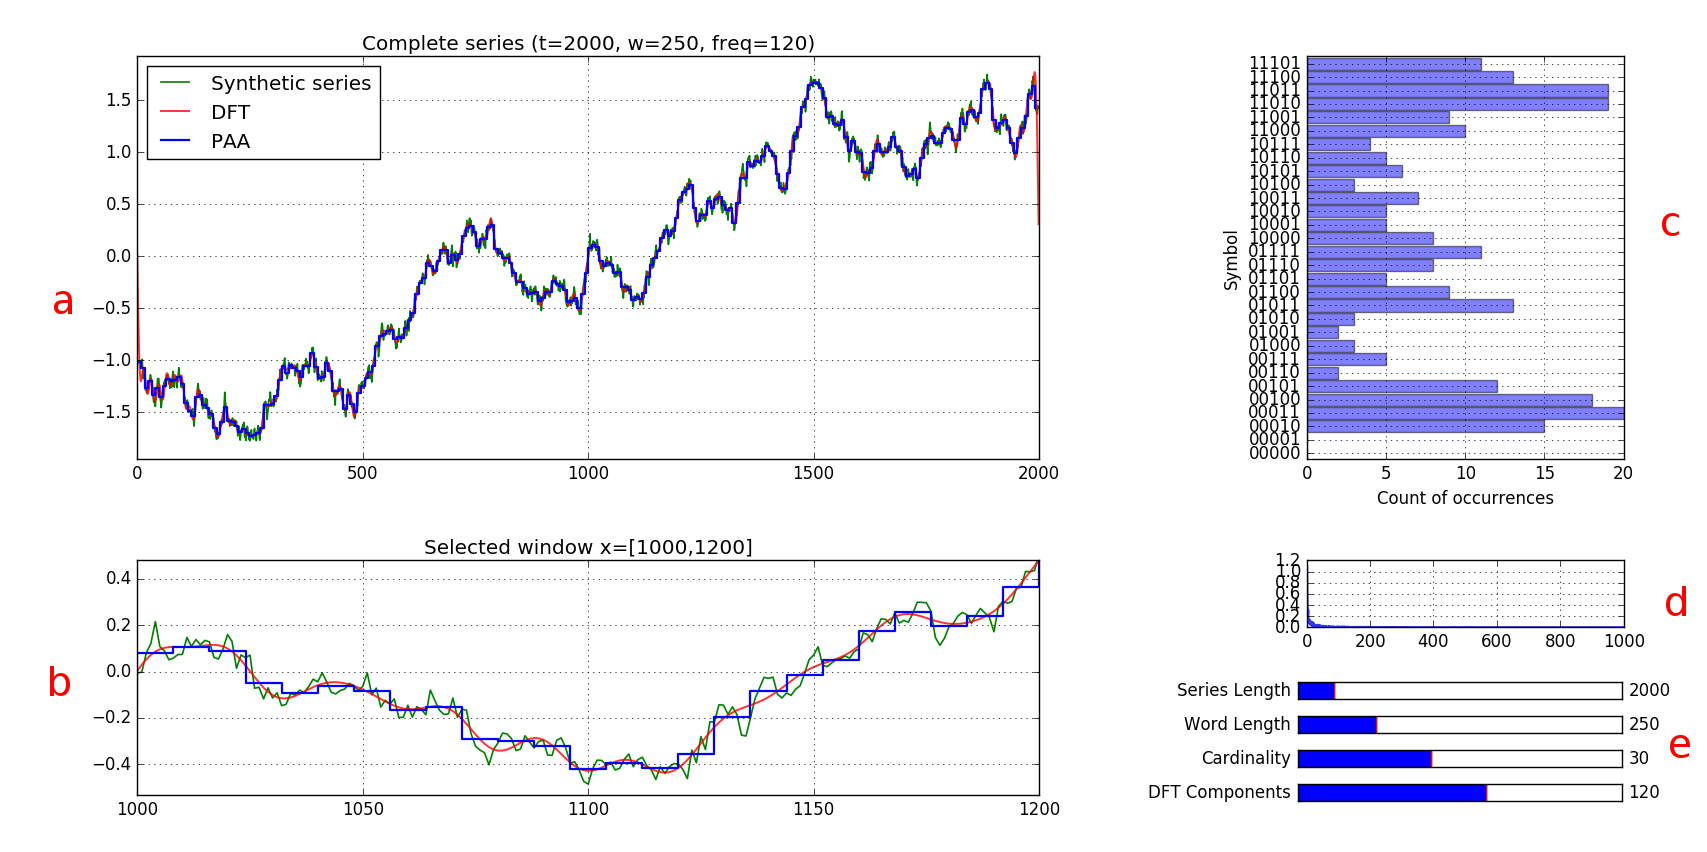
\includegraphics[width=\textwidth]{images/vis-labeled.png}
		\caption{Interactive user interface showcase with next components: a) provides a complete view on the synthetic time series and its transformations and allows selection of a smaller window to be displayed in b b) zoomed in view of the selected window in a c) distribution of SAX symbols in the transformed representation d) values of DFT frequency coefficients e) sliders that control series length, word length of a PAA transform, SAX cardinality and DFT frequency components used for reconstruction}
		\label{fig:2}
	\end{center}
\end{figure}

\section{Conclusions}
- sax is cool
- application scope
- there seems to be a need of data normalization into a [0, 1] to d domain, which to an exent might defeat the purpose of scalability (e.g. online learning or stream processing tasks)
- further work should include detailed analysis of SAX based prediction in 2 papers


\bibliography{sax-acquaintance}
\bibliographystyle{plain}
\end{document}